%\documentclass[10pt]{letter}
%\usepackage[utf8]{inputenc}

%%%%%%%%%%%%%%%%%%%%%%%%%%%%%%%%%%%%%%%%%%%%%%%%%
% compile with LuaLatex
%%%%%%%%%%%%%%%%%%%%%%%%%%%%%%%%%%%%%%%%%%%%%%%%%%%%%%%
\documentclass[11pt]{report}
\usepackage{epsfig}
\usepackage{amssymb,amsmath,amsfonts}
\usepackage[activeacute,american]{babel}
%\usepackage[utf8]{inputenc}
\usepackage{subfiles}
\usepackage{cite}
\usepackage{csquotes}
\usepackage{esvect}
\usepackage[acronym,nonumberlist]{glossaries}
\renewcommand{\acronymname}{Nomenclature}
\usepackage{multicol}
\usepackage{caption} 
\usepackage{float}
\usepackage[
    math-style=ISO,      % Upper Case Greek is in italics
    bold-style=ISO,      % Bold math is in italics
    partial=upright,     % nabla and partial upright
    nabla=upright,
  ]{unicode-math}
\topmargin 1.2cm 
\textwidth 16.1cm
\textheight 22.5cm
\oddsidemargin 0.7cm
\setcounter{tocdepth}{5}
\addtolength{\voffset}{-2.4cm}
\addtolength{\hoffset}{-0.5cm}

\usepackage{setspace}
%\doublespacing
\onehalfspacing
\usepackage{caption}
 \captionsetup[figure]{labelfont={bf},name={Figura},labelsep=period}


%%%%%%%%%%%%%%%%%%%%%%%%%%%%%%% 
% citas
% \footnotetext{Mott, Robert L. Mecanica de Fluidos 6/e. Pearson educación, 2006.}
% \footnotetext{Pritchard, Philip J. Fox and McDonald’s Introduction to Fluid Mechanics (8th ed.). John Wiley $\&$ Sons. (2011).}
% \footnotetext{Munson, Bruce R., et al. "Fundamentals of Fluid Mechanics, John Wiley $\&$ Sons." Inc., USA (2006).}
%%%%%%%%%%%%%%%%%%%%%%%%%%%%%%% 

%%%%%%%%%%%%%%%%%%%%%%%%%%%%%%%%%
\begin{document}
\centering{ \textbf{\Large{Mec\'anica de fluidos}}}

\centering {\Large{2$^\circ$ semestre 2020: 541209-1}}
\vspace{1cm}

\flushleft{ \large \underline{\textbf{Pr\'actica 5: Sistemas de tuber\'ias}}}

%%%%%%%%%%%%%%%%%%%%%%%%%
\vspace{1cm}

\underline {Problema 1 (P. 6.61 White\footnote{footnotes working fine}):}
\vspace{0.2cm}

Agua a $20^\circ$C es bombeada a trav\'es de una tuber\'ia de $2000$\,ft desde el tanque $1$ al tanque $2$, tal como se presenta el la figura~\ref{fig:fig1}, a una raz\'on de $3$ pies$^3$/s. Si la tuber\'ia es de hierro d\'uctil de di\'ametro $6$\,in y la bomba tiene una eficiencia de $75\%$, ¿qué potencia requiere la bomba?

\begin{figure}[H]
\centering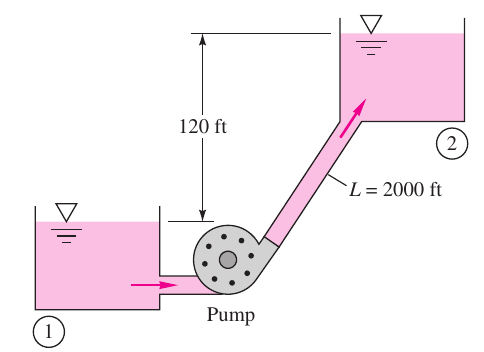
\includegraphics[width=0.5\textwidth]{Figures/p1.png}
\caption{\label{fig:fig1} }
\end{figure}

%%%%%%%%%%%%%%%%%%%%%%%%%
\newpage

\underline {Problema 2 (P. 6.105 White):}
\vspace{0.2cm}

El sistema de la figura~\ref{fig:fig3} cosiste de $1200$\,m de tuber\'ia de hierro d\'uctil de di\'ametro de $5$\,cm, dos codos a $45^\circ$ de radio largo y cuatro codos a $90^\circ$ de radio largo. Si la eleviaci\'on del punto $1$ es $400$\,m, que presi\'on manom\'etrica se requiere en el punto $1$ para que exista un flujo volum\'etrico de agua a $20^\circ$ de $0.005$\,m$^3/s$.

\begin{figure}[H]
\centering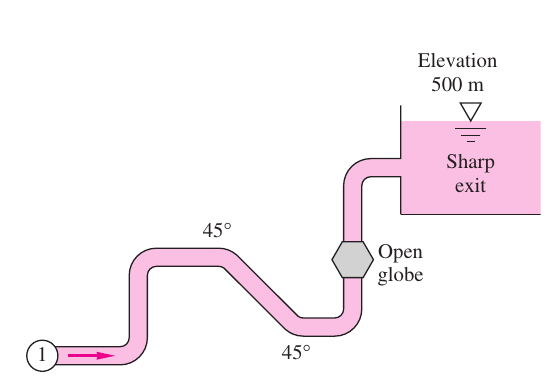
\includegraphics[width=0.5\textwidth]{Figures/p3.png}
\caption{\label{fig:fig3} }
\end{figure}

\footnotetext{F. M. White, “Fluid Mechanics,” 7th Edition, McGraw- Hill, New York, 2011.}




%%%%%%%%%%%%%%%%%%%%%%%%%
\underline {Problema 3 (P. 6.106 White):}
\vspace{0.2cm}

La tuber\'ia representada en la figura~\ref{fig:fig2} tiene un \'angulo de inclinaci\'on de $30^\circ$, d\'iametro de $1$\,in y es lisa. La v\'alvula de globo se encuentra completamente abierta. Si el man\'ometro de mercurio muestra una deflecci\'on de $7$\,in, ¿C\'ual es el flujo volum\'etrico de agua a $20^\circ$C?. Considere $K_{valvula}=16$.

\begin{figure}[H]
\centering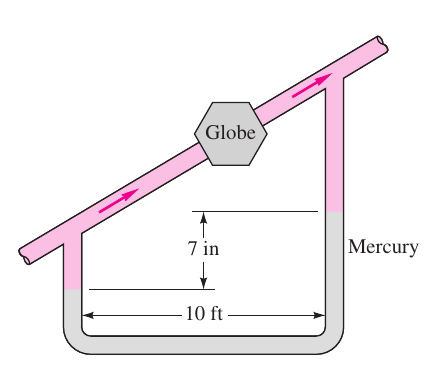
\includegraphics[width=0.5\textwidth]{Figures/p2.png}
\caption{\label{fig:fig2} }
\end{figure}


\underline {Problema 4 (P. 12.3 Mott\footnote{footnotes working fine}):}

Por el sistema de tubería ramificado que se aprecia en la figura~\ref{fig:fig4}, en el punto A circulan $850$\,L/min de agua a 10$^\circ$C, por una tubería de $4$ pulgadas, c\'edula 40. El flujo se bifurca en dos tuberías de $2$ pulgadas, c\'edula $40$, según se observa, y vuelve a unirse en el punto B. Calcule:
\vspace{0.2cm}

a) el flujo volumétrico en cada una de las ramas 

b) la diferencia de presión $p_A-p_B$. 
\vspace{0.2cm}

Incluya el efecto de las pérdidas menores en la rama inferior del sistema. La longitud total de la tubería de la rama inferior es de 60 m. Los codos son estándar.
\vspace{0.2cm}

\begin{figure}[H]
\centering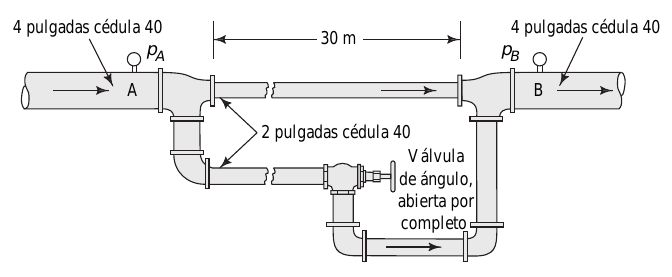
\includegraphics[width=0.8\textwidth]{Figures/p4.png}
\caption{\label{fig:fig4} }
\end{figure}

\footnotetext{Mott, Robert L. Mecanica de Fluidos 6/e. Pearson educación, 2006.}

%%%%%%%%%%%%%%%%%%%%%%%%%
\newpage
%%%%%%%%%%%%%%%%%%%%%%%%%
\underline {Problema 5 (P. 12.9 Mott):}
\vspace{0.2cm}

Encuentre el flujo volumétrico del agua a 60 °F en cada tuber\'ia de la figura~\ref{fig:fig5}


\begin{figure}[H]
\centering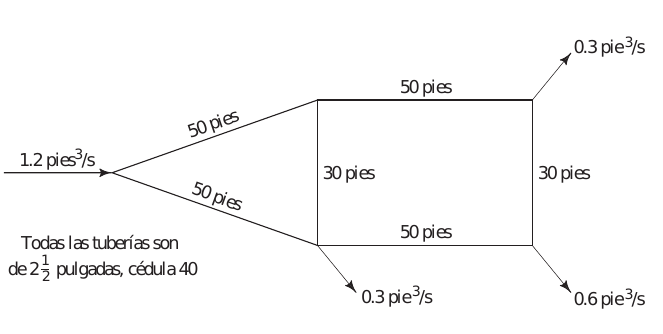
\includegraphics[width=0.8\textwidth]{Figures/p5.png}
\caption{\label{fig:fig5} }
\end{figure}

%%%%%%%%%%%%%%%%%%%%%%%%%
\newpage
%%%%%%%%%%%%%%%%%%%%%%%%%

\underline {Problema 6 (P. 12.11 Mott):}

La figura~\ref{fig:fig6} representa la red de distribución de agua de un parque industrial pequeño. El suministro de 15.5 pies$^3$/s de agua a 60$^\circ$F ingresa al sistema en el punto A. En los puntos C, E, F, G, H e I, plantas de manufactura extraen lo que se indica. Determine el flujo en cada tubería del sistema.

\begin{figure}[H]
\centering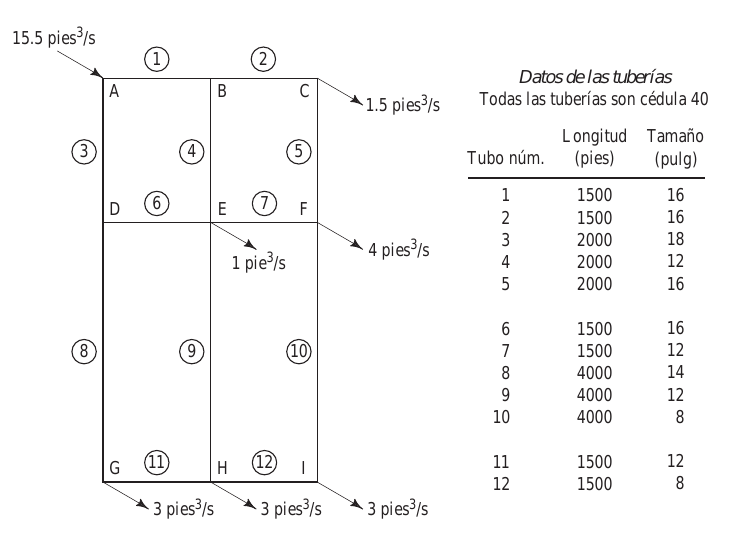
\includegraphics[width=0.8\textwidth]{Figures/p6.png}
\caption{\label{fig:fig6} }
\end{figure}
%%%%%%%%%%%%%%%%%%%%%%%%%
%%%%%%%%%%%%%%%%%%%%%%%%%
\end{document}
